\chapter{ÉTAT DE L'ART DE LA RECONNAISSANCE FACIALE }

\section{Introduction}
La mise en œuvre d'un système automatique et fiable de reconnaissance faciale est un verrou technologique qui n'est toujours pas résolu. Plusieurs études ont été menées à  ce sujet. Je présente dans ce chapitre un état de l'art sur les techniques les plus significatives de détection, puis de reconnaissance de visage. Enfin je ferai une synthèse des méthodes et techniques étudiées.

\section{Techniques de détection de visage}
\label{detection}
La détection de visage pose le problème de la localisation des visages présents dans une image d'entrée. Depuis quelques années, les recherches dans le domaine de la détection des formes, des objets ainsi que celle des visages s'intensifient et ont donné naissance à plusieurs techniques de détection de visages. Ces différentes techniques sont classifiées par Yang et al. dans \citep{Yan01} de la manière suivante :
\begin{itemize}
	\item \textbf{Méthodes basées sur les caractéristiques invariables} (feature invariant approaches) : \\
	Ces approches utilisent les éléments invariants aux variations d'illumination, d'orientation ou d'expression tels que la texture ou
la signature de couleur de la peau pour la détection.


	\item \textbf{Méthodes basées sur la connaissance} :
	
	Comme leur classe indique, les méthodes basées sur la connaissance (knowledge-based methods en anglais) utilisent les connaissances sur les différents éléments qui constituent le visage, ainsi que les relations existants entre eux. La classification "visage | non visage" est effectuée en mesurant les positions relatives de différents éléments clés tels que la bouche, le nez et les yeux. L'inconvénient de ces méthodes est qu'elles n'arrivent pas à détecter un visage sur un arrière plan complexe.
	
	
	\item \textbf{Méthodes basées sur la correspondance avec les modèles} ("template matching methods") :\\ 
	Pour ces méthodes, des modèles caractéristiques (templates) d'un visage ou de sous partie de visage sont créés. La localisation se fait ensuite en calculant la corrélation entre l'image candidate et le template. La corrélation peut être de deux types selon que le modèle est prédéfini ou déformable.
	
	\begin{itemize}
		\item Modèle prédéfini : 
		\item Modèle déformable : 
	\end{itemize}
	Ces méthodes ont l'inconvénient d'être sensibles aux variations de lumière, d'échelle.

\item\textbf{ Méthodes basées sur les apparences} (Appearence-based methods) : 
	Ces méthodes utilisent le même principe que présenté au point précédent mais se basent sur des modèles lus à partir des images d'entraînement(ou d'apprentissage). Le training set doit être constitué d'images représentatives et faites à différentes positions du visage. Les méthodes basées sur les apparences utilisent généralement les techniques d'analyse statistiques et d'apprentissage automatique pour décider de l'existence ou non d'un visage dans une image. Ces méthodes présentent l'avantage de s'exécuter très rapidement mais demandent un long temps d'entraînement. Elles sont les plus utilisées grâce à leur efficacité par rapport aux trois autres catégories de méthodes. Parmi ces méthodes, on peut citer l'algorithme de Viola et Jones \citep{VIO}, la méthode de Schneiderman et Kanade \citep{Kan} basée sur un classifieur de Bayes naïf, la méthode de Rowley et al. \citep{Row} basée sur les réseaux de neurones.
\end{itemize}
\subsection{Algorithme de Viola et Jones}
	Viola et Jones ont proposé en 2001 \citet{VIO} une méthode de détection de visage basée sur l'apparence. Première méthode de détection temps réel présentée, elle tourne à 15 fps pour des images de 384$\times$ 288 pixels sur un PC Intel Pentium III cadencé à 700Mhz. Le principe de cette  méthode  est d'obtenir  un  algorithme  complexe  de  classification,  composé  de classifieurs élémentaires qui éliminent au fur et à mesure les zones de l'image qui ne sont pas  compatibles  avec  l'objet  recherché. L'algorithme de Viola et Jones repose sur trois concepts clés : 
	\subsubsection{L'image intégrale}
	Dans le but d'extraire rapidement ces caractéristiques, Viola et Jones ont pensé une nouvelle forme de représentation de l'image : l'image intégrale. Sous cette forme, l'extraction d'une caractéristique à n'importe quel endroit et à n'importe quelle échelle est effectuée en un temps constant tandis que le temps de conversion vers la représentation intégrale ne remet pas en cause ce gain de temps. Pour localiser les visages présents dans l'image d'entrée, l'algorithme se base sur les caractéristiques de Haar \citep{VIO,MAT}. Dans toute image, une zone rectangulaire peut être délimitée et la somme des valeurs de ses pixels calculée. Une caractéristique de Haar est une simple combinaison linéaire de sommes ainsi obtenues. Plusieurs caractéristiques de Haar peuvent être définies selon le nombre, les échelles, les positions et les dimensions des zones rectangulaires considérées. La figure \ref{fig:haar} ci- dessous montre un exemple de quatre caractéristiques de Haar.
	
	\begin{figure}[htbp]
		\centering
			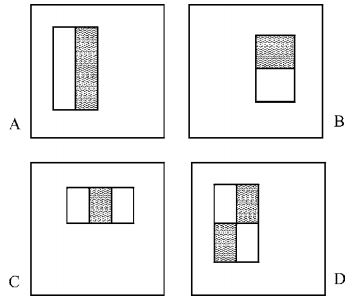
\includegraphics{haar.JPG}
		\caption[Exemple de 4 caractéristiques de Haar]{Exemple de 4 caractéristiques de Haar (source: \citep{VIO})}
		\label{fig:haar}
	\end{figure}
	
Le calcul d'une caractéristique de Haar requiert des accès aux valeurs de tous les pixels de la zone rectangulaire considérée. Quand le rectangle est de grande dimension, le calcul de la caractéristique devient contraignant temporellement. Pour pallier à cela, on fait appel à l'image intégrale ; Elle rend constant le calcul d'une caractéristique de Haar à n'importe quelle échelle.

L'image intégrale à l'emplacement $(x, y)$ dans une image contient la somme des images élémentaires au-dessus et à gauche de $(x, y)$ inclus : 
  \[ii(x, y)=\sum_{x'< x, y'< y }{i(x', y')}\] où $ii(x, y)$ est l'image intégrale et $i(x, y)$ l'image d'origine (voir figure \ref{fig:integr} ). 
	\begin{figure}[htbp]
		\centering
			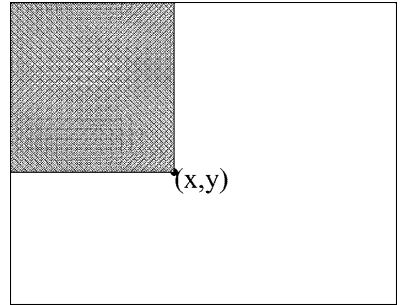
\includegraphics[height=175pt, width=175pt]{integr.JPG}
		\caption{image intégrale au point (x,y)}
		\label{fig:integr}
	\end{figure}
	
L'image intégrale est calculée rapidement en utilisant la paire de récurrences ci-dessous.
 \begin{eqnarray*}
s(x,y)=s(x,y-1)+i(x,y)\\
ii(x,y)=ii(x-1,y)+s(x,y)
\end{eqnarray*}
où $s(x,y)$ est la somme cumulative  des pixels sur une ligne. On a $s(x,-1)= 0$ et  $ii(-1,y) =0$.


Dans l'image intégrale, chaque pixel a pour valeur la somme des pixels se trouvant dans le rectangle supérieur gauche de l'image et lui même. Le calcul de la somme des valeurs des pixels d'une zone rectangulaire se fait en accédant seulement à quatre pixels de l'image qui sont les sommets de la zone rectangulaire. Soit la figure \ref{fig:rect} ci-dessous représentant une image intégrale.
\begin{figure}[htbp]
	\centering
		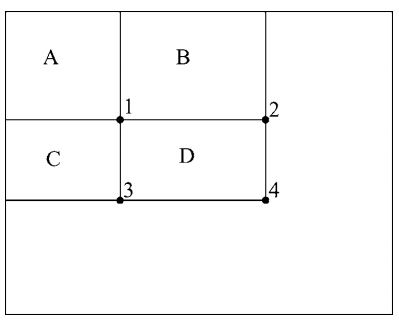
\includegraphics[height=175pt, width=175pt]{rect.JPG}
	\caption{calcul de la somme des pixels d'un rectangle}
	\label{fig:rect}
\end{figure}
Pour calculer la somme des pixels dans le rectangle D, on utilise uniquement les valeurs des pixels aux positions 1, 2, 3 et 4. La valeur du pixel en 1 est la somme des pixels du rectangle A. La valeur à la position 2 est A+B, à la position 3, elle est A+C, et à la position 4 elle est A+B+C+D. Ainsi on a : 
\begin{eqnarray*}
			4+1  & = &A+B+C+D+A \; (\; on\;  ajoute\;  A \; membre\;  à\;  membre\; )\\
			4+1  & = &2+3+D  \; (\; \; on \; réduit )\\
      D    & = &4+1-(2+3)\; (\; on\; tire D )
\end{eqnarray*}
														

	\subsubsection{Algorithme d'apprentissage basé sur Adaboost}
Pour localiser les visages sur l'image d'entrée, cette dernière est scannée par une fenêtre de dimension déterminée. La fenêtre parcourt l'image et son contenu est analysée pour vérifier l'existence ou non d'un visage. La classification est faite à l'aide des caractéristiques de Haar extraites de l'image et pour faciliter l'analyse, l'image est mise sous sa forme intégrale. Mais, pour une fenêtre de $24 \times 24$ pixels il y a 45 396 caractéristiques de Haar \citep{VIO}, les traiter toutes prendrait beaucoup trop de temps pour une application en temps réel. Pour surmonter ce problème, une variante de la méthode de boosting Adaboost est utilisée.

Je présente ci-dessous la méthode Adaboost ainsi que sa variante qui constitue le second apport de Viola et Jones.

Adaboost est une méthode d'apprentissage permettant de "booster" les performances d'un classifieur quelconque nommée "classifieur faible". L'idée est de faire passer les candidats à classifier à travers plusieurs classifieurs faibles, chacun étant entraînée en portant plus d'attention sur les candidats mal classifiées par le classifieur précédent.

Pour cela, des poids sont associées aux échantillons du training set

$((x_i; y_i) i = 1,\ldots ,m)$, tout d'abord de manière équilibrée :  


	\subsubsection{Cascade}
	
	Parmi l'ensemble des états de la fenêtre de recherche (c'est-à-dire les candidats) une partie peut être éliminée sur la base de l'évaluation de quelques caractéristiques de Haar : d'où le concept de cascade. Après élimination, les candidats restants sont analysés par des classifieurs forts, plus complexes demandant un plus grand temps de traitement. Cette manière de procéder évite donc d'effectuer des analyses lourdes en temps de calcul sur des échantillons pour lesquels il est rapidement possible de se rendre compte qu'ils sont négatifs. La classification apparaît donc comme une succession d'étapes où les échantillons classifiés positifs passent à l'étape suivante et les échantillons négatifs sont éliminés (voir figure \ref{fig:cacasde}).
	
	\begin{figure}[htbp]
		\centering
			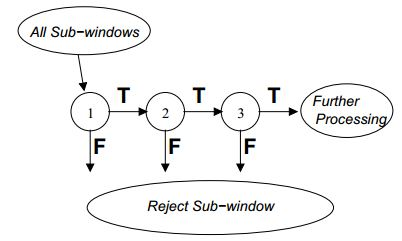
\includegraphics{cacasde.JPG}
		\caption[cascade de classifieurs forts]{cascade de classifieurs forts (source\citep{VIO})}
		\label{fig:cacasde}
	\end{figure}
	
	L'inconvénient de ce processus en cascade est que si le premier étage rejette un faux négatif, alors il ne sera plus jamais récupéré par la cascade. En d'autres termes le visage ne sera jamais détecté. Par contre si le premier étage transmet un faux positif, il pourra toujours être éliminée
aux étages suivants de la cascade.

Pour que la localisation soit rapide et atteigne des taux de détection élevés, les paramètres comme le nombre d'étages dans la	 cascade, leurs seuils de détection $\theta$ et le nombre de caractéristiques T considéré à chaque étage doivent être choisis convenablement. Ce choix doit être effectué pendant la construction de la cascade. 

L'entraînement de la cascade implique deux types de compromis : un classifieur avec un grand nombre de caractéristiques aura un taux élevé de détection et un faible taux de faux positifs, mais exigera un grand temps de calcul. Construire un classifieur avec le plus petit nombre possible d'étages dans la cascade, un nombre raisonnable de caractéristiques dans chaque étage et un meilleur taux de détection à chaque étage serait l'idéal. Malheureusement construire un tel classifieur reste un problème très difficile à résoudre.

Dans l'entraînement, une structure très simple est utilisée pour produire un classifieur effectif et très efficace. Chaque étape dans la cascade réduit le taux de faux positifs et diminue le taux de détection. Une cible est sélectionnée pour la réduction minimum des faux positifs et la baisse maximale de la détection. Chaque étape est entraînée en ajoutant des caractéristiques jusqu'à ce que la cible et les taux de faux positifs soient rencontrés (ces taux sont déterminés en testant le détecteur sur un ensemble de la validation). Les étapes sont ajoutées jusqu'à ce que la cible totale pour les faux positif et le taux détection soit rencontrée.

Le détecteur de visage développé par Viola et Jones dans \citep{VIO} est constitué de 38 étages et de plus de 600 caractéristiques. Néanmoins, elle opère rapidement. Sur un dataset difficile, contenant 507 visages et 75 millions de sous-fenêtres, les visages sont détectés après évaluation de 10 caractéristiques en moyenne  par sous-fenêtre. Ce système est approximativement 15 fois plus vite qu'une mise en œuvre du système de détection construit par Rowley et al. dans \citep{Row}.
Le tableau ci-dessous montre les performances de quelques algorithmes de détection de visage sur la base de données d'images MIT+CMU \footnote{MIT+CMU est une base de 130 images et 507 visages}.
 
\begin{table}[htbp]
	\centering
		\begin{tabular}{|l|c|c|c|c|c|c|c|}
			\hline	\backslashbox{d\'{e}tecteur}{faux positifs} & 10 & 31 & 50 & 65 & 78 & 95 & 167 \\
			\hline  Viola-Jones       & 76.1\% & 88.4\% & 91.4\% &92.0\% &92.1\%& 92.9\% &93.9\% \\
			\hline	Viola et Jones (Voting)& 81.1\% & 89.7\% & 92.1\% &93.1\% &93.1\%& 93.2\% &93.7\% \\
			\hline	Rowley-Baluja-Kanade   & 83.2\% & 86.0\% & -& - & - & 89.2\% & 90.1\%\\
			\hline	Schneiderman-Kanade     & - & -& - & 94.4\% & - & -  & -\\	
			\hline	Roth-Yang-Ahuja     & - & -& - & - & 94.8\%  &-   & -\\	
			\hline
		\end{tabular}
	\caption[taux de détection pour différents nombre de faux positifs sur la base d'image MIT+CMU]{taux de détection pour différents nombre de faux positifs sur la base d'image MIT+CMU}
	\label{tab:tauxDeDétection}
\end{table}
\subsection{Travaux améliorant l'algorithme de Viola et Jones}
\subsubsection{Nouvelle représentation intégrale}
  En plus de la représentation intégrale présentée plus haut, Lienhart et al. ont proposé une représentation intégrale inclinée où chaque pixel a pour valeur la somme des valeurs des pixels compris dans la zone rectangulaire inclinée de 45\degres dont le point extrême droit est le pixel considérée. Aux modèles initiaux de Viola et Jones sont donc ajoutés leurs équivalents inclinés de 45\degres. Les auteurs ont ainsi obtenu des améliorations de l'ordre d'un demi-pourcent.
	
	\begin{figure}[htbp]
		\centering
			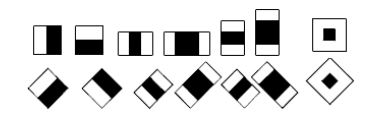
\includegraphics{haaram.JPG}
		\caption[représentation intégrale inclinée]{représentation intégrale inclinée (source : \cite{MAT}) }
		\label{fig:haaram}
	\end{figure}
	
	\subsubsection{Améliorations du Training set}
	Ayant constaté que l'on pouvait améliorer les performances du classifieur en préparant le set d'entraînement, Chen et al. \citep{CHEN} proposent une méthode basée sur un algorithme génétique pour étendre le set de visages. Selon eux leur approche est la plus prometteuse  dans le domaine de l'optimisation du Training set.
	
\section{Méthodes de reconnaissance de visages}

Une multitude de techniques de reconnaissance de visage ont été développées ces vingt dernières années.  L'identification  de  visage  est  un  axe  de  recherche  ouvert  attirant  des  chercheurs venants  de  disciplines  différentes  :  psychologie,  reconnaissance  de  formes, réseaux neuraux, vision artificielle et infographie. Le but ultime de la reconnaissance automatique de visage est  de  rivaliser,  voir  même  dépasser,  les  capacités  humaines  de reconnaissance. Nous allons détaillé dans cette partie quelques méthodes de reconnaissance faciale.

\subsection{Méthodes globales ou holistiques}
Les méthodes globales sont celles qui identifient un visage en prenant l'image entière de ce dernier comme entrée du système de reconnaissance \citep{Sou12}. Chaque image de visage de dimension $(n,m)$ est représentée 
par un vecteur simple de dimension $n\times m$, en concaténant les valeurs du niveau de gris de tous les pixels  de l'image du visage. L'avantage de cette représentation est qu'elle préserve implicitement les informations de texture et de forme nécessaire pour la reconnaissance de visages, mais nécessite une grande dimension de l'espace image. 

Ainsi, une image $100\times 100$, par exemple, est représentée par un vecteur de dimension $10^4$. Or le nombre d'images d'apprentissage pour chaque personne doit être au moins égal à dix fois la dimension du vecteur \citep{Jai}, il faut $10^5$ images  par  personne, ce qui serait difficilement réalisable en pratique.  Des techniques de réduction de  dimension sont généralement employées. Je présente ci-dessous les techniques de réduction par ACP et ADL.

\subsubsection{Analyse en Composante Principale (ACP) }

L'algorithme  PCA (Principal Component Analysis) est né des travaux de M. Turk et P. Pentland au MIT Media 
Lab, en 1991\citep{TURK}. L'ACP est une méthode mathématique qui peut être utilisée pour simplifier un ensemble de données en réduisant sa dimension. Elle permet ainsi de représenter efficacement les images de visage, qui peuvent approximativement être reconstruites à partir d'un petit ensemble de poids et d'une image de visage standard. Ces poids sont obtenus en projetant l'image du visage dans un espace de visage engendré par les visages propres.

La méthode \og eigenface \fg{} est l'une des méthodes basées sur l'ACP les plus utilisées \citep{Sou12}. Son principe est le suivant : étant donné un ensemble d'images de visages exemples, il s'agit tout d'abord de trouver les composantes principales de ces visages. Les visages propres (eigenfaces) sont des visages de même taille que les images d'apprentissage et qui montrent des visages ayant un aspect assez particulière (voir figure \ref {fig:eigenface}). Du point de vue mathématique, il s'agit des composantes principales de la distribution des visages, ou les vecteurs propres (eigenvectors) de la matrice de covariance de l'ensemble des images du visage. Chaque image du training set peut être représenté comme combinaison linéaire des visages propres et du visage moyen \citep{TOLBA}.
\begin{figure}[htbp]
	\centering
		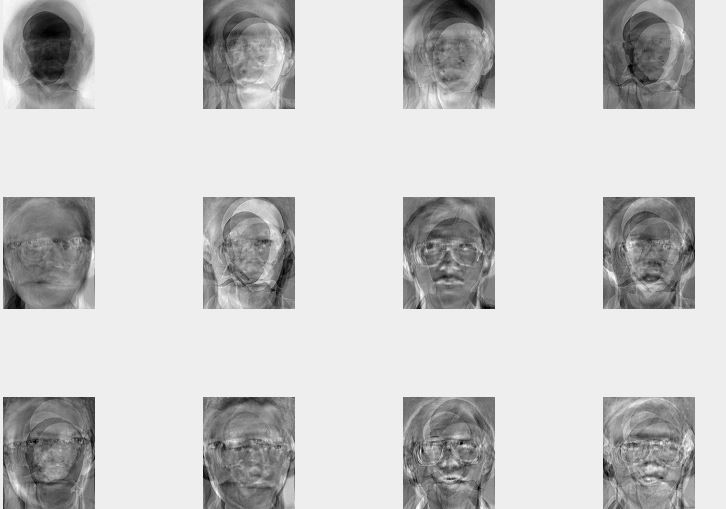
\includegraphics[height=250pt, width=400pt]{eigenface.JPG}
	\caption{exemple de faces propres}
	\label{fig:eigenface}
\end{figure}

Le nombre de visages propres est égal au nombre de visage dans le training set. Néanmoins, on peut réduire les calculs en ne considérant que les "meilleurs" eigenfaces (les meilleurs eigenfaces sont ceux ayant les plus larges valeurs propres qui représentent la plupart de variance dans l'ensemble des images de visage). L'ensemble  
de ces meilleurs eigenfaces forme le " Low Dimensional Space".
Le nombre d'images d'apprentissage influence sur les performances de l'algorithme eigenfaces. Pour illustrer cela, Wang et al. dans \citep{WAN} ont utilisé la base de données ORL\footnote{La base de données ORL 
contient des images de 40 individus, chacun étant enregistré sous 10 vues différentes.} comme base de test. Il ressort de leur étude que les performances de la méthode eigenface baisse avec la diminution du nombre d’exemples d'apprentissage pour chaque personne.  Dans le cas extrême, si le training set contient seulement une image, le taux d'identification moyen de l'eigenface tombe en dessous de 65 \%. Ce taux atteint 95\% quand on utilise neuf exemples d'apprentissage par personne. 


\subsubsection{Processus de reconnaissance par Eigenfaces}
Le processus de reconnaissance s'effectue en deux phases : la phase d'apprentissage et la phase de vérification.
La phase d'apprentissage  comprends dans l'ordre : 

\begin{itemize}
	\item [\textbullet]l'acquisition, la lecture et la normalisation des images des visages d'apprentissages (de taille R),
	\item [\textbullet]le calcul du visage moyen de ces images,
	\item [\textbullet]la détermination de la matrice de covariance $L=S^tS$ où $S$ est une matrice dont les colonnes sont les images obtenues après soustraction du visage moyen de chaque visage d'apprentissage normalisée,
	\item [\textbullet]le calcul des vecteurs propres $V$ et des valeurs propres $D$ de la matrice de covariance,
	\item [\textbullet]le calcul des visages propres (eigenfaces) selon la formule $U=S\times V\times (abs(D))^\frac{-1}{2}$,
	\item [\textbullet]Enfin le calcul des poids des visages de la base (de taille M) en les projetant dans le sous-espace engendré par les visages propres.
\end{itemize} 
   
Pendant la phase de vérification, on fait l'acquisition, la lecture et la normalisation de l'image de vérification (de taille R). Puis on soustrait le visage moyen de l'image normalisée. Ensuite on calcule le poids de l'image en utilisant les images propres comme une base de projection. Enfin on mesure la similarité en utilisant la distance euclidienne. %\citep{}.

L'ACP est une technique rapide, simple et populaire dans l'identification de modèle, c'est l'une des meilleures techniques. Cependant, l'ACP n'est pas optimisée pour la séparabilité (discrimination) de classe aux dépens de l'analyse discriminante linéaire (LDA). 

\subsubsection{Analyse Discriminante Linéaire (ADL)}

L'algorithme LDA est né des travaux de Belhumeur et al. De Yale University (USA), en  1997 \citep{BEL}. Il est aussi connu sous le nom de \og Fisherfaces \fg{}. Les méthodes basées sur l'Analyse Discriminante Linéaire  déterminent les directions de projection les plus discriminantes dans l'espace engendré par les visages propres. Pour cela, elles maximisent les variations inter-personne par rapport aux variations intra-personne. Pour utiliser la technique LDA, l'on doit préalablement organiser la base d'apprentissage en plusieurs classes : en raison d'une classe par personne et plusieurs images par classe.  La LDA analyse les vecteurs propres de la matrice de dispersion des données, avec pour  objectif de maximiser les variations entre les 
images d'individus différents (interclasses) tout  en minimisant les variations entre les images d'un même individu (intra-classes). Cependant, si un seul exemple d'apprentissage par personne est utilisé, c'est-à-dire
si les variations intra classes nulles, alors les performances de l'ADL deviennent faibles par rapport à celles  qui sont données par l'eigenface \cite{MAR}.

Plusieurs autres méthodes ont été développées ces dernières années à l'instar de la méthode eigenface probabiliste, la méthode de la Machine Vecteur Support (SVM), la méthode de la ligne caractéristique, la méthode Laplacianfaces. Ces méthodes sont généralement plus performantes que la méthode eigenface basique \cite{Sou12}, mais lorsque le training set est constitué d'une seule image, certaines de ces méthodes se réduisent à l'eigenface basique ou peuvent ne plus fonctionner.

Les méthodes holistiques souffrent du problème du petit nombre d'échantillon (small size sample problem)qui dégrade leurs performances. Néanmoins des méthodes surmontant ce défaut comme (PC)$^2$A \citep{WU}, sa généralisation E(PC)$^2$A \cite{SONG} et la 2DPCA \citep{JIAN} ont été développées. Des stratégies visant à étendre le training set peuvent être également utilisées (utilisation des images symétriques gauches et droites pour générer de nouvelles vues, la méthode de déformation parallèle pour générer de nouvelles poses à partir d'une première photo). 
\subsection{Méthodes locales}
Les méthodes locales utilisent les caractéristiques faciales locales pour la reconnaissance de visage. Cette catégorie se divise en deux sous-catégories basées respectivement sur des caractéristiques et des apparences locales.
\subsubsection{Méthodes basées sur l'apparence locale}

Les méthodes basées sur l'apparence locale utilisent en entrée plusieurs vecteurs correspondant aux caractéristiques du visage à reconnaître. Elles sont utilisées de manière modulaire pour les différentes régions du visage. Un modèle global est alors défini par la combinaison de plusieurs modèles locaux. De cette façon, les différentes régions du visage ne sont pas affectées de la même manière par les différentes sources de vulnérabilités. Ces méthodes sont à priori mieux adaptées pour le problème à échantillon
unique \cite{XIAO}.
\subsubsection{Méthodes basées sur des caractéristiques locales}
Les méthodes basées sur les caractéristiques locales peuvent être classées en deux catégories: les approches géométriques et les approches basées sur les graphes.

Pour des approches géométriques, des propriétés géométriques sont extraites à partir de la localisation de points clés sur le visage (tel que le nez, la bouche et les yeux).
Un exemple est le système décrit par Brunelli et Poggio \citep{BRU}  qui extrait automatiquement 35 caractéristiques géométriques du visage et qui utilise les classifieurs de Bayes pour calculer la similitude. Pour ce système, les auteurs ont enregistré un taux d'identification de 90\% sur une base de données de 47 sujets. Le  coût  de  stockage  des  techniques géométriques est très bas comparé à celui des autres techniques. Toutefois, les méthodes purement géométriques présentent deux principaux inconvénients qui sont :
\begin{itemize}
	\item la localisation des points clés qui n'est pas toujours chose facile lorsque les occlusions ou variations d'expressions ou de pose surviennent,
	\item  l'information nécessaire à une reconnaissance robuste n'est pas forcement contenue dans ces quelques points clés.
\end{itemize}

Comme exemple de méthodes locales, nous avons la méthode des Local Binary Patterns, la méthode EBGM \cite{EBGM} (Elastic Bunch Graph Matching), etc.

Le tableau ci-dessous (tirée de \cite{Sou12}) est une comparaison entre les méthodes basées sur les deux types de caractéristiques.
\begin{table}[htbp]
	\centering
		\begin{tabular}{|l|l|l|}
			\hline
			Facteurs de variation & Caractéristiques locales& Caractéristiques globales\\
			\hline illuminations & très sensible& sensible\\
			\hline expressions & pas sensible& sensible\\
			\hline pose & sensible& très sensible\\
			\hline bruit & très sensible& sensible\\
			\hline occlusions & pas sensible& très sensible\\
			\hline
		\end{tabular}
	\caption{comparaison des méthodes basées sur les caractéristiques globales ou locales} 
	\label{tab:comparaison}
\end{table}
\subsection{Méthodes hybrides}
Comme leur nom indique, les méthodes hybrides sont celles qui combinent les méthodes globales et locales. Le but est de bénéficier des avantages de l'un et de l'autre. La combinaison efficace entre caractéristiques locales et globales reste pour le moment un problème et peu de travaux sur son application au problème de la reconnaissance faciale existent \citep{XIAO}.

Le tableau \ref{tab:scoresDeCertaines} extrait de \cite{Beymer}montre les performances des méthodes les plus performantes dans le domaine de la reconnaissance faciale à partir d'une seule image par personne.

\begin{table}[htbp]
	\centering
		\begin{tabular}{|l|p{2cm}|p{1cm}|p{1cm}|p{2cm}|p{3cm}|}
			\hline
			\footnotesize méthode&\footnotesize BD d'images& \footnotesize personnes de test&\footnotesize images de test& \footnotesize score le plus élevé/score de base& \footnotesize facteurs de variation \\ \hline
		\footnotesize Parallel deformation&\footnotesize N/A&62&620&\footnotesize 85.0/ 32.1&\footnotesize Pose\\ \hline
		\footnotesize Local probalistic subspace& \footnotesize AR&100&600&\footnotesize 82.5/ 70.2& \footnotesize Expression, temps\\ \hline
		\footnotesize Someface& \footnotesize AR&100&600&\footnotesize 93.7/ 70.2&\footnotesize Expression, temps\\ \hline
			\footnotesize 2DPCA& \footnotesize AR&100&600& \footnotesize 74.8/ 70.2&\footnotesize Expression, temps\\ \hline
			\footnotesize ID-DDHM&\footnotesize AR&120&1440&\footnotesize 89.8/ 27.2&\footnotesize Expression, illumination, temps\\ \hline
			\footnotesize (PC)$^2$A&\footnotesize FERET&200&200&\footnotesize 83.5/83.0&\footnotesize N/A\\ \hline
		\footnotesize E(PC)$^2$A&\footnotesize FERET&200&200&\footnotesize 85.5/ 83.0&\footnotesize N/A\\ \hline
		\footnotesize SDV perturbation&\footnotesize FERET&200&200&\footnotesize 85.0/ 83.0&\footnotesize N/A\\ \hline
		\footnotesize Modular FLDA&\footnotesize FERET&200&200&\footnotesize 86.5/ 83.0&\footnotesize N/A\\ \hline
		\footnotesize Component LDA&\footnotesize FERET&70&350&\footnotesize 78.6/ 32.0&\footnotesize Expression, illumination, temps\\ \hline
		\footnotesize EBGM&\footnotesize FERET&1196&1196&\footnotesize 95.0/ 79.7&\footnotesize Expression\\ \hline
		\footnotesize LBP&\footnotesize FERET&1196&1196&\footnotesize 97.0/ 79.7&\footnotesize Expression\\ \hline
		\footnotesize Discriminant PCA&\footnotesize FERET&256&914&\footnotesize 72.0/ 74.0&\footnotesize Expression,temps\\ \hline
		\footnotesize Analytic-to-hilistic approch&\footnotesize ORL&40&160&\footnotesize 84.0/ 74.7&\footnotesize Pose\\ \hline
		\footnotesize face specific subspace&\footnotesize Yale&15&150&\footnotesize 95.3/74.7&\footnotesize Expression,illumination\\ 
			\hline
		\end{tabular}
	\caption[algorithmes et leurs performances sur le 'one sample problem']{scores de certaines méthodes s'attaquant au problème de la reconnaissance faciale avec des training sets composés d'un seul échantillon par personne}
	\label{tab:scoresDeCertaines}
\end{table}


\section{Conclusion} 
Dans ce chapitre, nous avons présenté un ensemble de techniques de détection et de reconnaissance de visages. L'
engouement  pour  les  systèmes  de  reconnaissance  des  visages  est  justifié  par  les  nombreux
avantages de cette approche.